\section{Distribution of Potential and Kinetic Energy of Bound Particles after a Finite Time}
\label{sec:DistributionPotKinEnBound}
The viral theorem states the following relation for the kinetic energy $E_{kin}$ and potential energy $E_{pot}$ of a bound gravitational system in equilibrium. 
\begin{align}
	2\left< E_{kin} \right> = - \left< E_{pot} \right>
	\label{eq:ViralTheorem}
\end{align}
$\left< E_{kin} \right>$ and $\left< E_{pot} \right>$ represents the time average of the kinetic and potential energy, respectively, but by the ergodic hypothesis, this can be made the ensamble average. \fxnote{cite!}

To study whether the viral theorem of \matref{eq:ViralTheorem} is fulfilled with the computed algorithms, the final kinetic and potential energy of the bound particles of a system initially consisting of 70 particles after a time period of $\tau_{crunch}$.
It is expected that the fraction of the mean of the kinetic energy and the mean of the potential energy will be close to $-2$, even though it in \secref{sec:StabilityAndEquilibrium} is found that the equilibrium is not reached before than after a time period of $2\tau_{crunch}$. 

In addition, to get rid of some of the numerical instabilities, a smoothing function, as argued for in \secref{sec:argumentforepsilon}, is introduced.
To check the consistency with the Viral theorem of the fourth order Runge-Kutta method when including the smoothing function, similar histograms for the distribution of the kinetic energy and potential energy after a finite time period as shown in \figref{fig:DistributionPotKinEnBoundHistograms} is generated to determine the mean of the kinetic energy and potential energy.
The bound particles are found by the same argument as in \fxnote{ref to magnus-sec} that a particle is bound if the total energy of that particle is negative, that is the particle is bound if the absolute value of the potential energy is greater than the absolute value of the kinetic energy.
\begin{figure}[H]
\centering
\begin{minipage}{.5\textwidth}
  \centering
  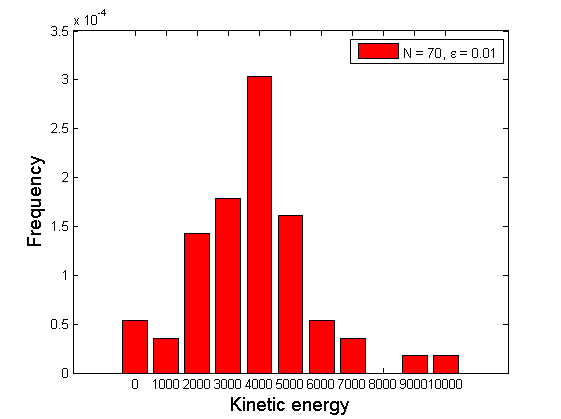
\includegraphics[width=1\linewidth]{Figures/Histograms_including_epsilon/N_70_e_n3_kin.png}
\end{minipage}%
\begin{minipage}{.5\textwidth}
  \centering
  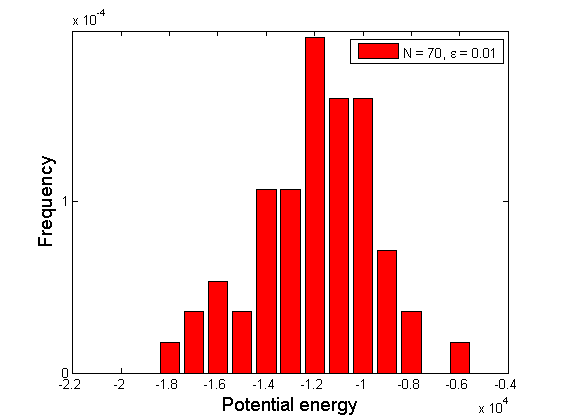
\includegraphics[width=1\linewidth]{Figures/Histograms_including_epsilon/N_70_e_n3_pot.png}
\end{minipage}
\caption{
	Distribution of the kinetic and potential energy of bound particles in the star cluster after a time period of $1\tau_{crunch}$ with a step length of $1\times 10^{-4} \tau_{crunch}$ and $\epsilon = 1\times 10^{-2} \text{ ly}$ for 70 particles with normal distributed masses, uniformly distributed within a sphere generated by the functions presented in \secref{Method:GeneratingPosMassVel}. 
}
\label{fig:DistributionPotKinEnBoundHistograms}
\end{figure}
The kinetic and the potential energy of the bound particles seem to follow a more or less uniform distribution after a finite time period. 
This is also seen when computing histograms for different values of $\epsilon$. 
The mean of these distributions for the kinetic energy and potential energy after are shown in the table below for various values of $\epsilon$. 